\section{Old Trilogy}
\epigraph{''Do or do not. There is no try''}{\textasciitilde Yoda}

\subsection{Episode \texorpdfstring{\rom{4}}{4} -- A New Hope}
\lipsum[1-2]
\subsection{Episode \texorpdfstring{\rom{5}}{5} -- The Empire Strikes Back}
\lipsum[2-3]
\subsection{Episode \texorpdfstring{\rom{6}}{6} -- Return of the Jedi}
\lipsum[3-4]

\section{New Trilogy}

\begin{figure}[ht]
\centering
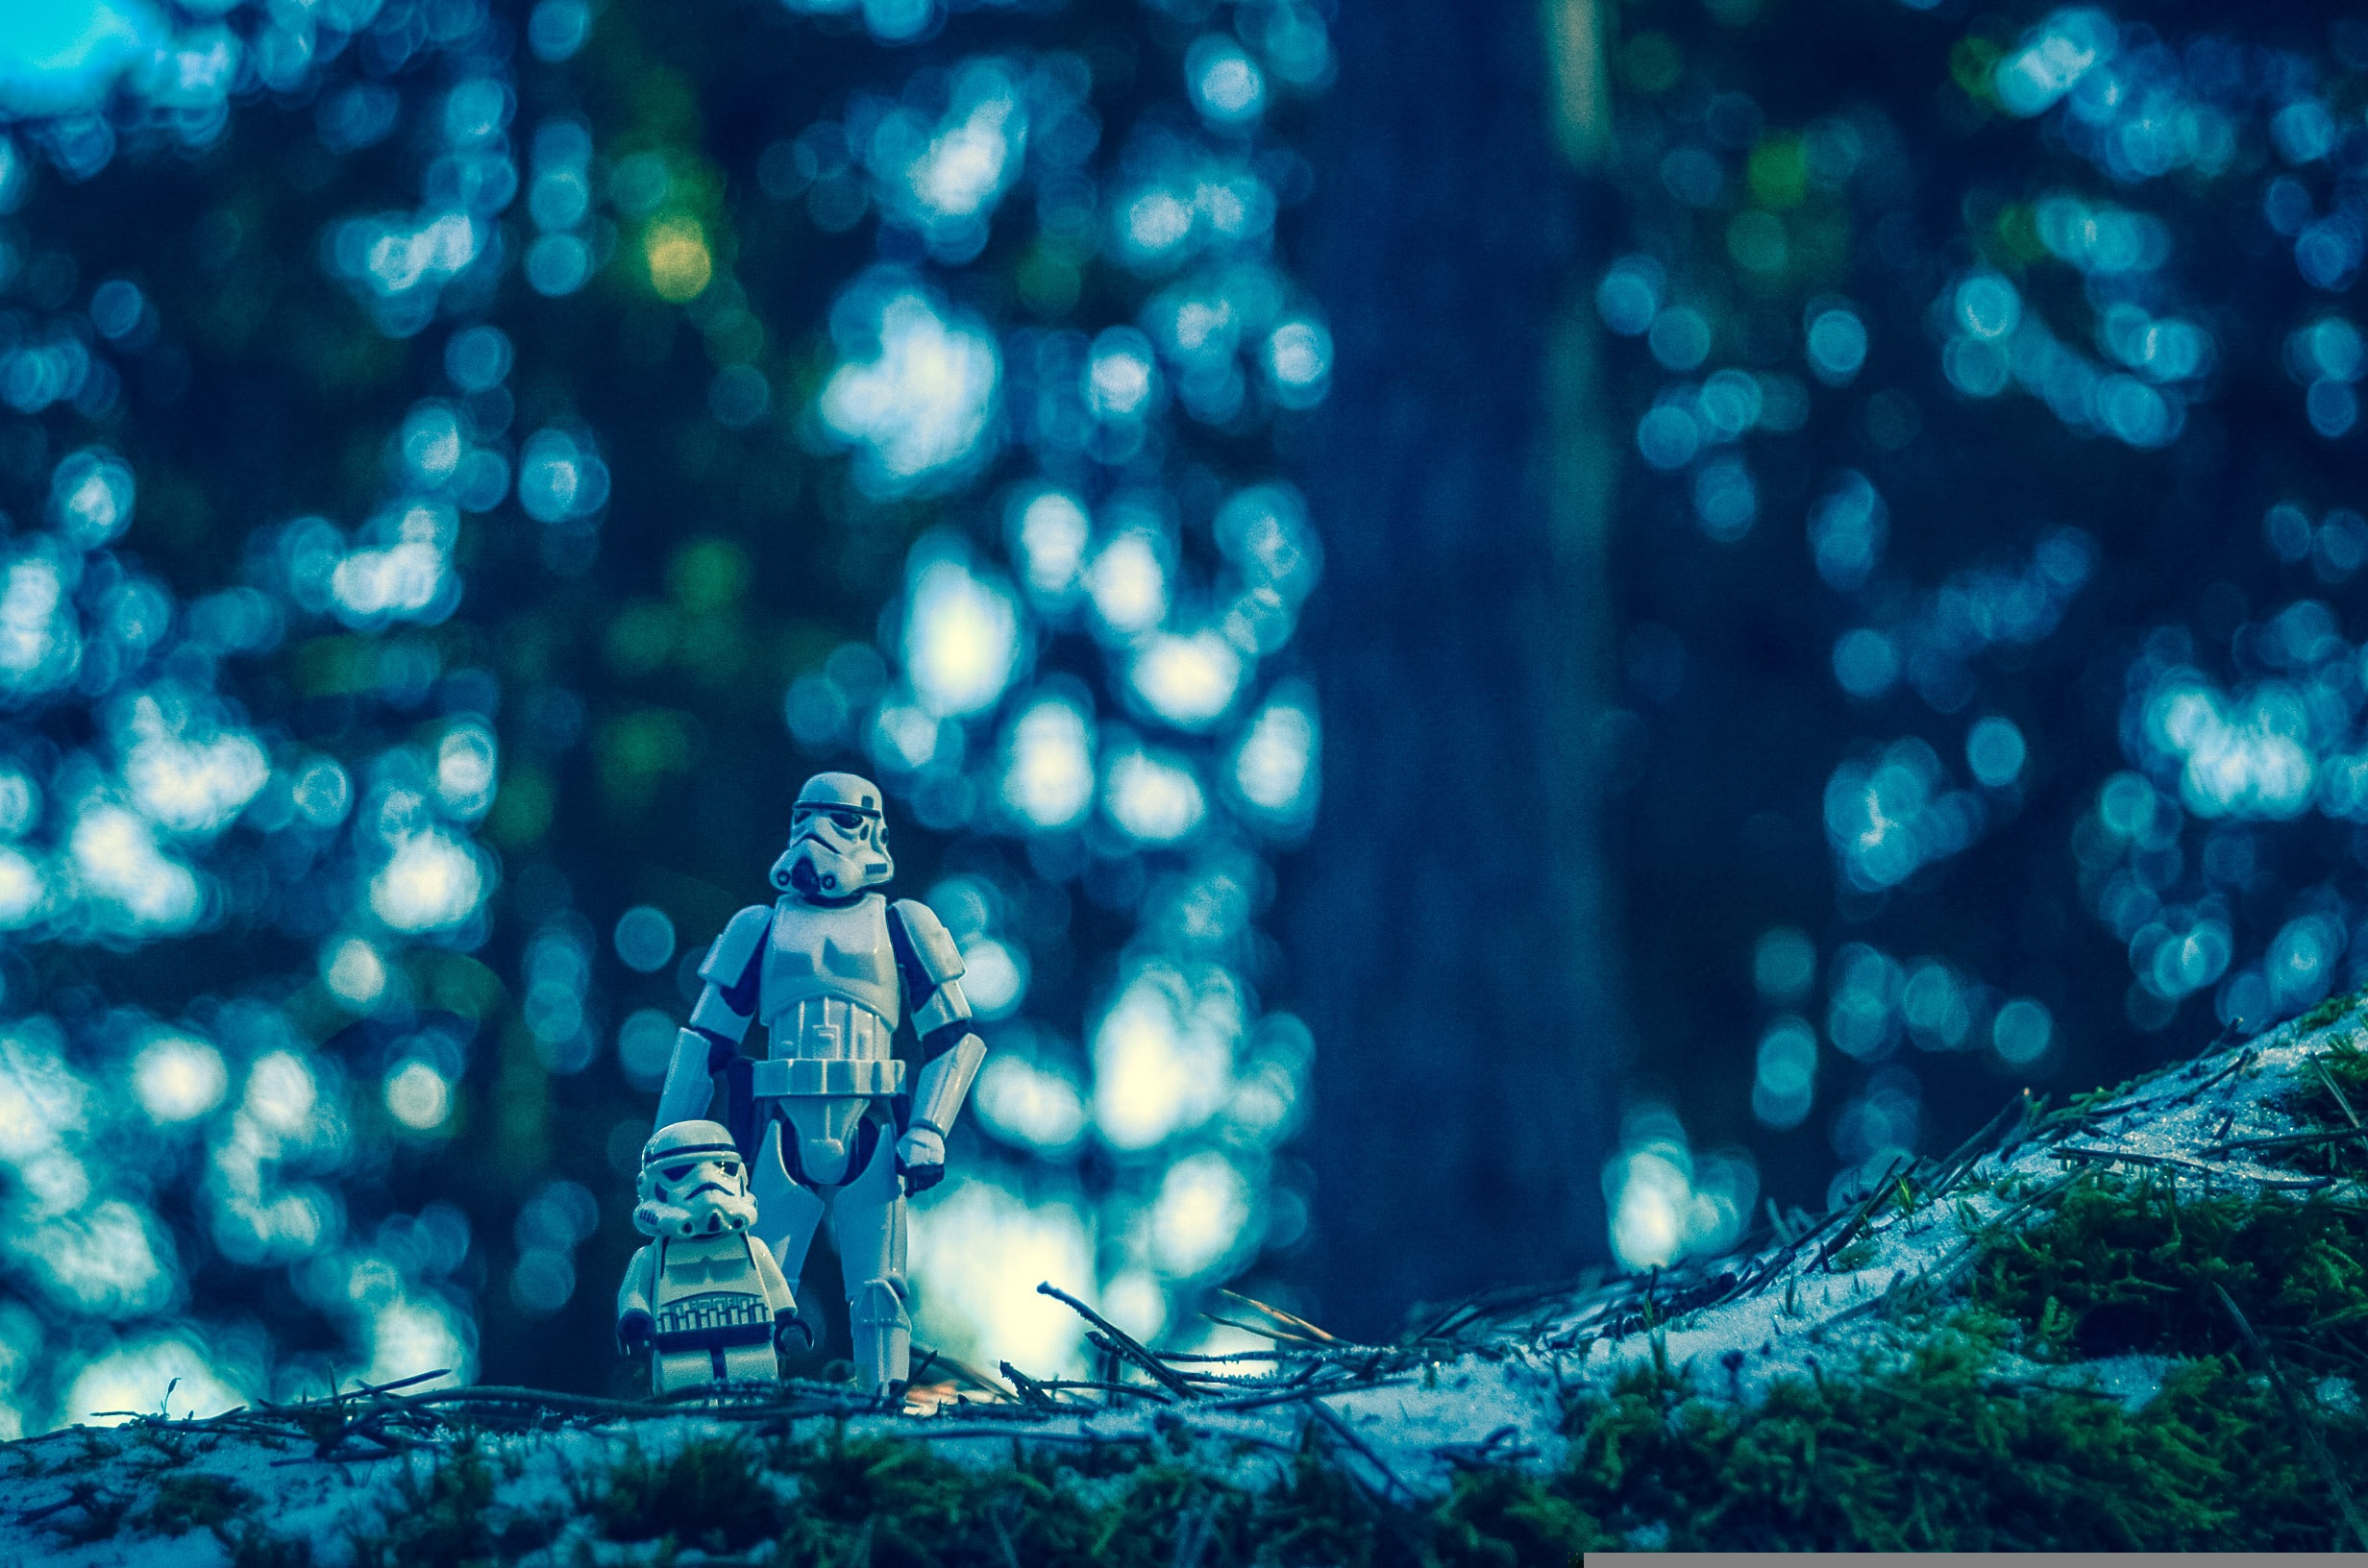
\includegraphics[width=\textwidth]{sturmtruppler.jpg}
\caption{Stockimage von \cite{trooper}}
\label{fig:trooper}
\end{figure}

\subsection{Episode \texorpdfstring{\rom{1}}{1} -- The Phantom Menace}
\lipsum[1-2]
\subsection{Episode \texorpdfstring{\rom{2}}{2} -- Attack of the Clones}
\marginpar{\footnotesize \raggedright The origin of ''Across the stars''. A wonderful piano version\cite{piano} exists on \url{https://www.youtube.com/watch?v=lFuhQXn1WhQ}}
\noindent\lipsum[2-2]
\subsection{Episode \texorpdfstring{\rom{3}}{3} -- Revenge of The Sith}
\lipsum[3-4]
